\chapter{Introduction to Packings}

\scribe{Ferran Dachs Cadefau}

The general content of the lectures.

\section{Packings}

\begin{defn}
 A family $\{K_i\}_{i\in I}$ of compact convex sets $K_i\subseteq\RR^d$ with non-empty interior (this implies that $K_i$ are full-dimensional) is a \textit{packing} if:

$$\interior(K_i\cap K_j)=\emptyset\qquad \text{for }i\neq j $$
\end{defn}

It is possible that the boundaries of two different $K_i$ overlap, but not the
interior. If we are working in a Hausdorff space, subsets are compact if and only if they
are closed and bounded. More generally, we can work with  non-convex packings, but they are
harder to work with. For example the next example due to M.C. Escher:
\begin{figure}[htbp]
  \centering
  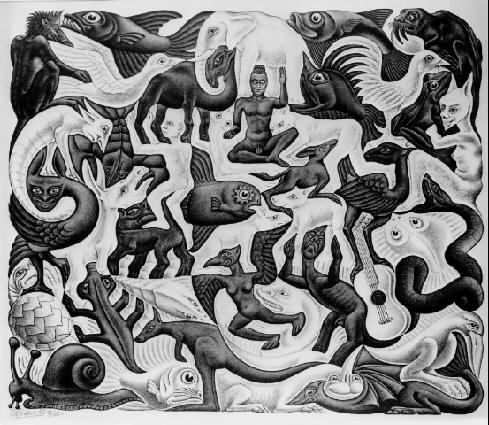
\includegraphics[width=.5\linewidth]{Escher}
  
  \caption{M.C. Escher, Plane Filling II, Lithograph 1957}
\label{fig:intro:1}
\end{figure}

\begin{defn}
  If there exists $C\in\RR^d$ such that $\bigcup_{i\in I}K_i\subseteq C$
  then $C$ is called a \emph{container} of the packing. These always exist:  take $C=\bigcup_{i\in I}K_i$.
  The \emph{natural container} of the packing is
$$C_{nat}=\conv \displaystyle{\bigcup_{i\in I}K_i}$$
\end{defn}

We will pack repetitions of the same figure, that is, $K_i$ for all $i\in I$ is the same
set. Another thing that we can consider is a fixed container: For example, we can pack
squares in squares as in \cite{Friedman}, or circles in squares, as in
\url{http://hydra.nat.uni-magdeburg.de/packing/csq/csq.html}, or regular polyhedra
\cite{Jaoshvili}. As we can see in the second example, if we have a fixed container it is
hard to find a optimum solution, and moreover, the optimum solution can have no
regularity!

\begin{defn}
 We can speak about the quality of the packings using their \emph{density}
 \[
   \delta_{bin}
   \ = \
   \frac{\sum_{i=1}V(K_i)}{V(C)}
\]
and \emph{natural density}
\[
   \delta_{Nat}
   \ = \
   \frac{\sum_{i=1}V(K_i)}{V(C_{Nat})}.
\]
\end{defn}

From now on, the $K_i$ will be congruent spheres.

\section{Density of disk packings in the plane}



\begin{lemma}[Thue in 1892]
 $$\delta_{Nat}(n \text{ disks in }\RR^2)\underset{n\rightarrow\infty}{\longrightarrow}\delta_{Nat}(\text{hexagonal packing})$$
 $$\delta_{Nat}(n \text{ thin disks in }\RR^3)=1$$
 where thin disks are: $D^2\times\square^1$ and the ideal packing is a cylinder. For bigger dimensions (thin disks are: $D^2\times\square^{d-1}$) the ideal packing is again a cylinder. 
\end{lemma}

\section{Packings of Spheres}

\begin{obs}
 We defined: $S^d=\left\{x\in\RR^{d+1}:\|x\|=1\right\}$.
 Except for $S^0$ all spheres are connected, and all $S^i$ for $i>1$ are simply connected.
\end{obs}

\begin{defn}
 Let $Z=\conv\left\{\text{centers of }K_i: i\in I\right\}$. We say that the
 associated packing is a 
\begin{enumerate}
 \item \emph{Sausage} if $\dim Z=1$;
 \item \emph{Pizza} if $2\leqslant\dim Z\leqslant d-1$;
 \item \emph{Pile} if $\dim Z=d$.
\end{enumerate}
\end{defn}

For example, in $\RR^2$ a Sausage is composed of $n$ circles with their centers on a
line. In $\RR^3$, we get a Pizza for example by thinking of $n$ spheres with their centers
on a plane.
\[
  \delta_{Nat}(\text{Sausage of }n\text{ spheres in }\RR^d)
  \ = \ 
  \frac{\sum_{i=1}V\left(K_i\right)}{V\left(\conv\bigcup_{i\in I}K_i\right)}
  \ = \
  \frac{n\beta(d)}{\beta(d)+2(n-1)\beta(d-1)},
\]
where $\beta(d)$ are the volume of the unit ball in $\dim d$. To calculate the volume of
$\conv\bigcup_{i\in I}K_i$ we have used that the convex hull is a cylinder of
height $n-1$ and two halves of a sphere.

\[
  \delta_{Nat}(\text{Sausage of }n\text{ spheres in }\RR^d)
  \ \underset{n\rightarrow\infty}{\longrightarrow}\ 
  \frac{\beta(d)}{2\beta(d-1)}.
\]

\begin{figure}[htbp]
  \centering
  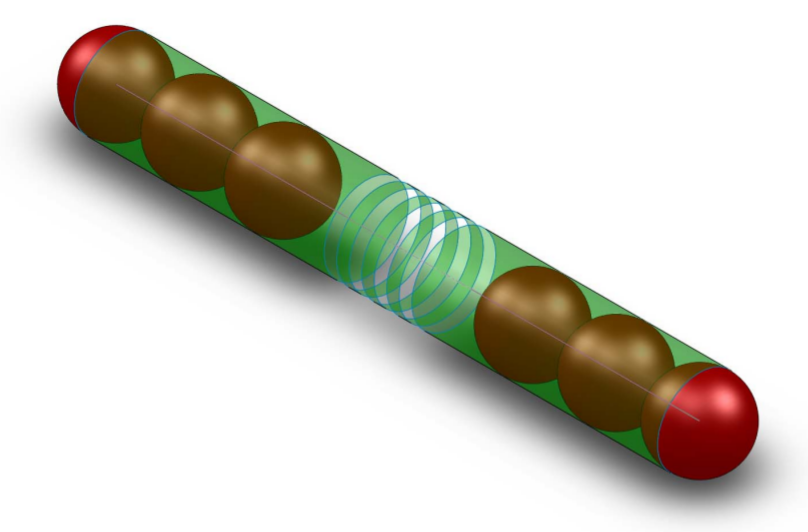
\includegraphics[width=.5\linewidth]{sausage_28_10}
  
  \caption{Sausage in $\RR^3$ with its natural density $C_{Nat}$.}
\label{fig:intro:2}
\end{figure}

For example the case $n=4$ and $d=3$ the best packing is a Sausage instead of for example the Tetrahedral packing as we can see in The paper of J.M.Wills.

\begin{exercise}
 Calculate the $\delta_{Nat}$ of the tetrahedral packing.
\end{exercise}

In dimension $3$ the best packings are shown in Table~\ref{tab:packings-dim3}.


\begin{table}[htbp]
  \centering
  \begin{tabular}{p{4cm}||c|c|c|c|c|c|c|c|c|c|c|c|c}
   $n$
   (number of balls) &4&...&55&56&57&58&59&60&61&62&63&64&$\geqslant65$\\
   \hline\hline
   Type of best packing &S&...&S&P&S&S&P&P&P&P&S&S&P\\
   \hline
   Verified or Conjectured&V&C&C&V&C&C&V&V&V&V&C&C&V
 \end{tabular}
 
\medskip
 \caption{Best packings in dimension 3. 
   Here  $S$ stands for Sausage, $P$ for Pile, $C$ is Conjectured and $V$ is Verified.}
\label{tab:packings-dim3}
\end{table}


\begin{conj}[Sausage Conjecture (L\'aszlo Fejes T\'oth)]
 $$\delta(d,n)=\delta_{Nat}(W_n^d) \qquad \forall n\in \NN, \quad d\geqslant 5$$

Where $W_n^d$ is the sausage packing (``Wurst'' in German).
\end{conj}

\begin{theorem}[Martin Henk, J\"org Wills, Ulrich Betke 1986; see \cite{Betke-Henk}]
 $$\delta(d,n)=\delta_{Nat}(W_n^d) \qquad \forall n\geqslant42, \quad d\geqslant 5$$
\end{theorem}

\section{The Unit cube}

Now, we can consider $\square^d$, the unit cube in $\RR^d$:
\[
   \square^d
   \ = \ 
   \conv\{(a_1,...a_d)|a_i=0\text{ or }1, \text{ for }0\leqslant i\leqslant
   d\}\subseteq\RR^d
\]

\begin{figure}[htbp]
  \centering
  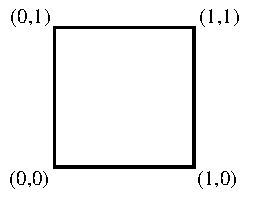
\includegraphics[width=.2\linewidth]{unit_cube_d2}
  
  \caption{$\square^2$}
\label{fig:intro:3}
\end{figure}

\begin{obs}
 The number of vertices of $\square^d$ is $2^d$.
\end{obs}

\begin{defn}
 $$\square^d=\left\{(a_1,...a_d)|0\leqslant a_i\leqslant 1 \quad \forall 0\leqslant i\leqslant d\right\}\subseteq\RR^d$$
 We can consider the faces of $\square^d$, and his \textit{dimension} are the dimension of his affine span. 
\begin{itemize}
 \item If dimension are $0$ we talk about \textit{vertices}.
 \item If dimension are $1$ we talk about \textit{edges}.
 \item If dimension are $d-1$ we talk about \textit{facet}.
\end{itemize}

\end{defn}

\begin{obs}
 The number of facets of $\square^d$ is $2d$, one for each inequality.
\end{obs}

\begin{exercise}
 Calculate all the number of dimension $i$ subspaces.
\end{exercise}

\begin{obs}
  The distance between a vertex and the barycenter is the radius of the
  \emph{circumscribed sphere}. If $V$ is a vertex, and $B$ the barycenter, we have:
$$\|V_i-B\|=\|(0,...,0)-(1/2,...,1/2)\|=\|(1/2,...,1/2)\|=\sqrt{d}\frac{1}{2}$$
 We can choose $V=(0,...,0)$ because all vertices are at the same distance from the barycenter.

\begin{figure}[htbp]
  \centering
  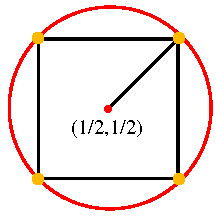
\includegraphics[width=.2\linewidth]{squarecirc}
  
  \caption{The distance between a vertex and the barycenter is the radius of the circumscribed sphere.}
\label{fig:intro:4}
\end{figure}
\end{obs}

\begin{obs}
 The distance between a facet and the barycenter is the radius of the \emph{inscribed sphere}, $\frac{1}{2}$.
\begin{figure}[htbp]
  \centering
  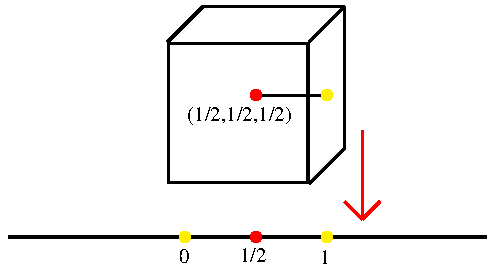
\includegraphics[width=.4\linewidth]{projsquare}
  
  \caption{The distance between a facet and the barycenter is the radius of the inscribed sphere, $\frac{1}{2}$}
\label{fig:intro:5}
\end{figure}
\end{obs}

Here we show the radii of the circumscribed and the inscribed spheres in some dimensions:
$$\begin{array}{c|c|c|c|c}
   d&1&2&100&10^4\\
   \hline
   &&&&\\
   \rho_{circ}&\frac{1}{2}&\frac{1}{2}\sqrt{2}&5&50\\
   &&&&\\
   \hline
   &&&&\\
   \rho_{in}&\frac{1}{2}&\frac{1}{2}&\frac{1}{2}&\frac{1}{2}\\
   &&&&\\
  \end{array}
$$
\begin{figure}[htbp]
  \centering
  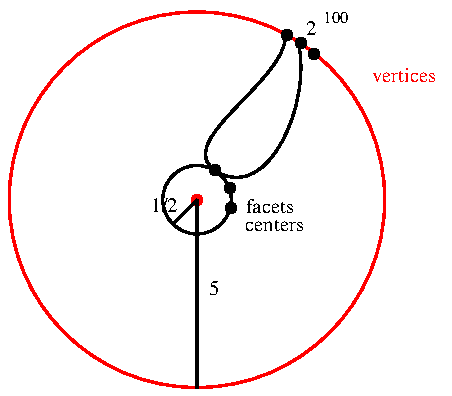
\includegraphics[width=.3\linewidth]{square100}
  
  \caption{Representation of the vertices and the facets in dimension $100$. }
\label{fig:intro:6}
\end{figure}

It's difficult to think in high dimensions. For more, see \cite{Ball}.

\begin{obs}
 If we draw $2^d$ spheres centered in the vertices with radius $\frac{1}{2}$. Which is the radius of the maximum sphere that we can draw centered in the barycenter tangent to the others (as we can see in Figure \ref{fig:intro:7})? $\frac{1}{2}\left(\sqrt{d}-1\right)$

$$\begin{array}{c|c|c|c|c|c}
   d&2&3&4&5&100\\
   \hline
   &&&&&\\
   \frac{1}{2}\left(\sqrt{d}-1\right)&0.2&<\frac{1}{2}&\frac{1}{2}&>\frac{1}{2}&\frac{9}{2}\\
   &&&&&\\
  \end{array}
$$

In the table we can see that in dimensions over $5$ the sphere goes out the facets!
\end{obs}

\begin{figure}[htbp]
  \centering
  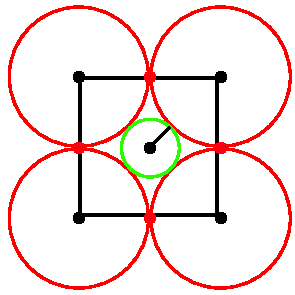
\includegraphics[width=.23\linewidth]{squareintcirc}
  
  \caption{Representation of the vertices and the facets in dimension $100$.}
\label{fig:intro:7}
\end{figure}

% Local Variables: 
% mode: latex
% TeX-master: "dag-upc"
% End: 
